\chapter*{Základní definice}
\label{sec:zakladni-pojmy}
\addcontentsline{toc}{chapter}{Základní definice}

\begin{definition}[Polytop]
  \emph{Polytop} dimenze $n \in \mathbb{N}$ je uzavřená podmnožina $P \subseteq \R^{n}$ definovaná induktivně:
  \begin{itemize}
    \item Polytop dimenze $1$ je úsečka.
    \item Polytop dimenze $n$ je slepením polytopů dimenze $n-1$, jež spolu mohou
          sdílet stěny libovolné dimenze, kde \emph{stěnou} polytopu rozumíme jeho
          libovolnou podmnožinu jsoucí rovněž polytopem.
          Zároveň neexistuje nadrovina (podprostor dimenze $n - 1$), která by obsahovala všechny jeho vrcholy.
          \autocite{adamklepacDefinicePolytopu2024}
  \end{itemize}

\end{definition}

\begin{definition}[Bod]
  \label{definice:bod}
  Bod je uspořádaná $n$-tice $(\xx{1}, \xx{2}, \ldots, \xx{n}) \in \R^n$. Ve $2D$ budu používat značení $a=(a_x, a_y)$.
\end{definition}

\begin{definition}[Vzdálenost]
  \label{definice:vzdalenost}
  Zobrazení $d: \R^n\times \R^n~\rightarrow~\R^+$ nám určí vzdálenost dvou bodů $u, v \in \R^n$
  podle předpisu $d(u, v) \coloneqq \sqrt{(\vvv{1}-\uu{1})^2+(\vvv{2}-\uu{2})^2+\ldots+(\vvv{n}-\uu{n})^2}$.
\end{definition}

\begin{definition}[Ohodnocený graf]
  \label{definice:ohodnoceny_graf}
  $G = (V, E, w)$ je ohodnocený graf, kde $V$ je množina vrcholů, $E$ je množina dvouprvkových podmnožin $E \subseteq \binom{V}{2}$ a $w$ je libovolné zobrazení $E \rightarrow \R^+$, které hranám přiřazuje jejich váhu.
\end{definition}

\begin{definition}[Úplný ohodnocený graf]
  \label{definice:uplny_ohodnoceny_graf}
  Úplný ohodnocený graf $G = (V, E, w)$ má kaž\-dé dva vrcholy spojeny hranou, neboli $E = \binom{V}{2}$. Takový graf můžeme také zapsat jako $K_n \coloneqq (V,\binom{V}{2},w)$.
  \begin{figure}[h]
    \centering
    \begin{subfigure}[b]{0.3\textwidth}
      \centering
      \begin{tikzpicture}
        \graph { subgraph K_n [n=3, clockwise, radius=0.3\textwidth, nodes={font=\small}] };
      \end{tikzpicture}
    \end{subfigure}
    \begin{subfigure}[b]{0.3\textwidth}
      \centering
      \begin{tikzpicture}
        \graph { subgraph K_n [n=5, clockwise, radius=0.3\textwidth, nodes={font=\small}] };
      \end{tikzpicture}
    \end{subfigure}
    \begin{subfigure}[b]{0.3\textwidth}
      \centering
      \begin{tikzpicture}
        \graph { subgraph K_n [n=7, clockwise, radius=0.3\textwidth, nodes={font=\small}] };
      \end{tikzpicture}
    \end{subfigure}
    \caption{Úplné grafy $K_3$, $K_5$ a $K_7$}
    \label{obr:uplne_ohodnocene_grafy}
  \end{figure}
\end{definition}

\begin{definition}[Podgraf]
  \label{definice:podgraf}
  Graf $H = (V', E')$ je podgraf grafu $G = (V, E)$, pokud $V' \subseteq V$ a $E' \subseteq E \cap \binom{V'}{2}$.
\end{definition}

\begin{definition}[Cesta]
  \label{definice:cesta}
  Cestou v grafu nazveme posloupnost \textbf{různých} vrcholů $v_1, \ldots, v_n$, pokud $\forall i \in \{1,\ldots, n-1\}$ platí $\{v_i, v_{i+1}\} \in E$.
\end{definition}

\begin{definition}[Váha cesty]
  \label{definice:vaha_cesty}
  Pokud cestu tvoří posloupnost vrcholů $v_1, \ldots, v_n$, tak váha cesty je rovna \[ w(\{v_1,\dots ,v_n\}) = \sum_{i=1}^{n-1}w(\{v_i, v_{i+1}\}). \]

\end{definition}

\begin{definition}[Cyklus]
  \label{definice:cyklus}
  Cyklus je posloupnost vrcholů $v_1,\ldots,v_n,v_1$, kde $v_1,\ldots,v_n$ je cesta a  $\{v_1,v_n\}$ je hrana v množině hran $E$.
\end{definition}

\begin{definition}[Váha cyklu]
  \label{definice:vaha_cyklu}
  Pokud cyklus tvoří posloupnost vrcholů $v_1, \ldots, v_n$, tak váha \\cyklu je rovna \[ w(\{v_0,\dots ,v_n, v_0\}) = w(\{v_1, v_n\}) + \sum_{i=1}^{n-1}w(\{v_i, v_{i+1}\}). \]
\end{definition}

\begin{definition}[Soused]
  \label{definice:soused}
  V grafu $G = (V, E, w)$ je vrchol $u$ soused vrcholu $v$, pokud hrana $\{u, v\} \in E$.
\end{definition}

\begin{definition}[Trojúhelníková nerovnost]
  \label{definice:trojuhelnikova_nerovnost}
  Trojúhelníková nerovnost říká, že pro kaž\-dé tři různé body $a, b, c$ platí \textcolor{myblue}{$d(a, b)+d(c, b)$} $\geq$ \textcolor{myred}{$d(a,b)$}, neboli vzdálenost mezi dvěma body je vždy menší nebo rovna součtu vzdáleností mezi těmito body a třetím bodem.

  \begin{figure}[h]
    \centering
    \begin{tikzpicture}
      \label{obr:trojuhelnikova_nerovnost}
      \coordinate[label=below left:$a$] (A) at (0,0);
      \coordinate[label=below right:$b$] (B) at (6,0);
      \coordinate[label=above:$c$] (C) at (3,2);
      \draw[myred, line width=1.5pt] (A) -- (B);
      \draw[myblue, line width=1.5pt] (B) -- (C);
      \draw[myblue, line width=1.5pt] (C) -- (A);
      \fill (A) circle[radius=2pt];
      \fill (B) circle[radius=2pt];
      \fill (C) circle[radius=2pt];
    \end{tikzpicture}
    \caption{Trojúhelníková nerovnost}
  \end{figure}
\end{definition}

\begin{definition}[Obvod trojúhelníku]
  \label{definice:obvod_troj}
  Definujeme zobrazení $p: \R\rightarrow \R^+$ podle předpisu: $p(a, b, c) \coloneqq d(a, b) + d(b, c) + d(a, c)$, které nám určuje obvod $\Delta(a,b,c)$.
\end{definition}

\begin{definition}[Big $\mathcal{O}$ notation]
  \label{definice:bigonotation}
  Vizte například \autocite{Bae2019}. Krátce řečeno: notace $\mathcal{O}(\dots)$ představuje počet kroků, kolik algoritmus musí udělat v nejhorším případě. O algoritmu můžeme říct, že má časovou složitost například $\mathcal{O}(n^2)$.

  \begin{figure}[H]
    \centering
    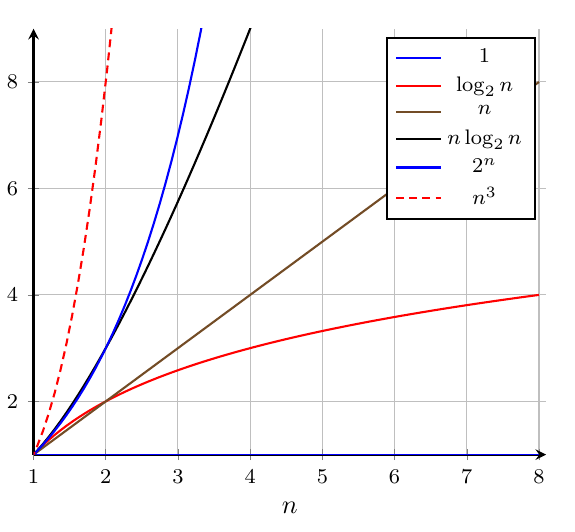
\begin{tikzpicture}[scale=0.95]
      \begin{axis}
        [
        axis lines = left,
        xmin=1, xmax=8.1, ymin=1, ymax=9,
        domain=0:8, samples=100, no markers, thick, grid=both,
        xlabel = \(n\), ylabel = {\(f(n)\)},
        label style = {overlay},       % Has he same effect as
        ticklabel style = {overlay},   % trim axis [left|right]
        legend entries = {
          $1$,
          $\log_{2}n$,
          $n$,
          $n\log_{2}n$,
          $2^{n}$,
          $n^{3}$,
        },
        every axis/.style = {font=\footnotesize},
        label style = {font=\normalsize},
        ]
        \addplot+ {1};
        \addplot+ {1 + ln(x)/ln(2)};
        \addplot+ {x};
        \addplot+ {1 + x*ln(x)/ln(2)};
        \addplot+ {2^x-1};
        \addplot+ {x^3};
      \end{axis}
      \coordinate[label=below:\phantom{a}] (A) at (5, -0.25);
    \end{tikzpicture}
    \caption{Grafy různých funkcí} \label{obr:big_o}
  \end{figure}
\end{definition}